The \TVB simulator resembles popular neural network simulators in 
many fundamental ways, both mathematically and in terms of informatics 
structures, however we have found it necessary to introduce auxiliary
concepts particularly useful in the modeling of large scale brain 
networks.

% need to cite Andreas' work and 

\subsection{Node dynamics}

	In our models, nodes are not abstract neurons nor necessarily 
	small groups thereof, but rather large populations of neurons, considered
	by, for example, the work of Wilson and Cowan. 

	\note[mw]{quick list of models \& their relevance}

\subsection{Network structure}
	
	The nodes are embedded in two scale network structure. The first of which
	is derived from empirical measurements of the myelinated corticocortical
	connectivity, which we shall refer to as the inhomogeneous, large scale
	structure. An implication of this structure is the inherent delays in 
	communication due to finite conduction velocity.

	The second form of network structure is prescribed in the case of a 
	cortical surface by the combination of said surface and a connectivity
	kernel. Together, these generate a homogeneous, local connectivity. 
	For the current work, we consider this coupling to be instantaneous.

	\note[mw]{Need to explain regional \& surface simulations}

\subsection{Integration of stochastic delay differential equations}

	Rather unlike other simulation paradigms, both noise and delays are
	common features of simulations in \TVB. As such, the simulator is equipped
	with Heun and Euler methods for stochastic integration and the pairwise
	inter-regional delays are treated in an efficient fashion. 

	\note[mw]{the general equation here}

	\note[mw]{Describe handling of delays?}

\subsection{Forward solutions}

	One of the primary goals of the \TVB simulator is to allow for the
	simulation of empirical whole-brain data, such as EEG or fMRI.
	\TVB implements several forward solutions as so-called monitors, 
	including MEG, sEEG, EEG and fMRI. 

	Crucially, given the amount of data \TVB may produce, especially for
	simulations on a cortical surface, each of the monitors is "on-line"
	in the sense that is runs in constant space.

\subsection{Native code generation for C \& GPU}

	Several of the core components (integrators, mass models, coupling
	functions) have targeted towards a C source code backend, which has
	allowed for the compilation of simulations to native code loaded 
	either as a shared library accessed via the \texttt{ctypes} modules
	or as CUDA kernels accessed via the \texttt{pycuda} module \cite{pycuda}.
	While such an approach may provide speed ups, they depend on the
	presence of a C compiler and, in the case of GPU, the CUDA toolkit and
	a compatible graphics card, and in the future, prepacked versions of \TVB
	will include precompiled objects for most kinds of simulations. 

	The approach used in compiling a simulation to native code takes advantage
	of the fact that CUDA is quite similar to C, and thus a generic template
	abstracts much of the boilerplate between the two. For each part of the 
	simulator, a generic function is customized with a class specific kernel;
	for example, in the case of a neural mass model, we have in the Python class

	\begin{lstlisting}
	class Generic2dOscillator(Model):
	    tau = FloatArray(...)
	    # etc.

	    device_info = model_device_info(
		pars=[tau, a, b, c, d, I],
		kernel="""
		float tau  = P(0)
		    , a    = P(1) ; // etc

		// state variables
		    , v    = X(0)
		    , w    = X(1)

		// aux variables
		    , c_0  = I(0)   ;

		// derivatives
		DX(0) = d * 
		(tau * (w - v*v*v + 3.0*v*v + I + c_0));
		DX(1) = d * 
		((a + b*v + c*v*v - w) / tau);
		"""
	    )
	\end{lstlisting}

	\noindent where the device\_info attribute is used to specify how the
	class's mathematical description fits into the general model function:

	\begin{lstlisting}
	/* wrapper for model specific code computing RHSs of diff-eqs */
	__device__
	void model_dfun(
	  float * _dx, float *_x, float *mmpr, float *input)
	{
	#define X(i) _x[n_thr*i]
	#define DX(i) _dx[n_thr*i]
	#define P(i) mmpr[n_thr*i]
	#define I(i) input[i]

	    // begin model code
	    \$model_dfun
	    // end model specific code

	#undef X
	#undef DX
	#undef P
	#undef I
	\end{lstlisting}

	\noindent where the C preprocessor defines allow the model specific
	kernel to easily reference the correct parts of the multidimensional 
	per-thread arrays (in the case of the GPU). 

	 \begin{figure}
		{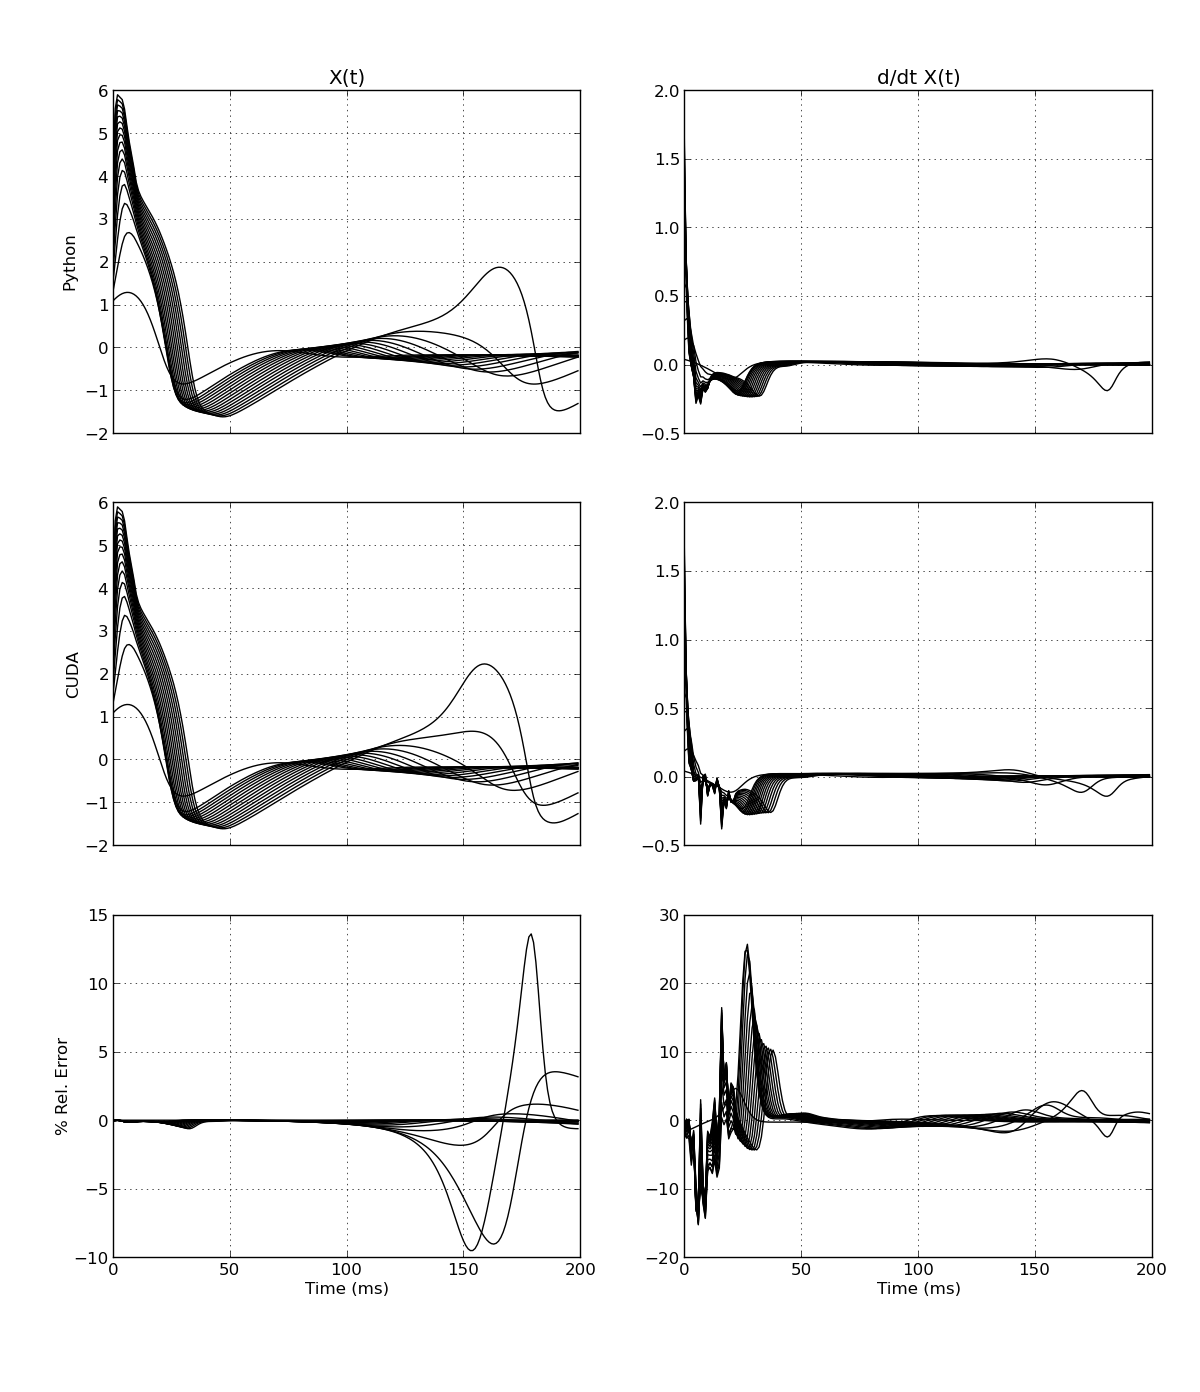
\includegraphics[width=0.48\textwidth]{images/gpu_dxdt.png}}
		\caption{
		Right A typical parameter space exploration, 32 x 32 grid of
		coupling strength (y-axis) v. neural excitability (x-axis).
		This grid of simulations was run on both TVB's Python/NumPy
		implementation and the new GPU backend for 200 ms simulation
		time with otherwise default parameters. The former took ~2
		hours and the latter ~ 1 min. Left Quantitative comparison of
		solutions and instantaneous derivatives is shown for an even
		sampling of the parameter space across k where a = -2, because
		this slice showed the most error on the GPU. 	
		}
		\label{fig:gpu_dxdt}
	\end{figure}

	 \begin{figure}
		{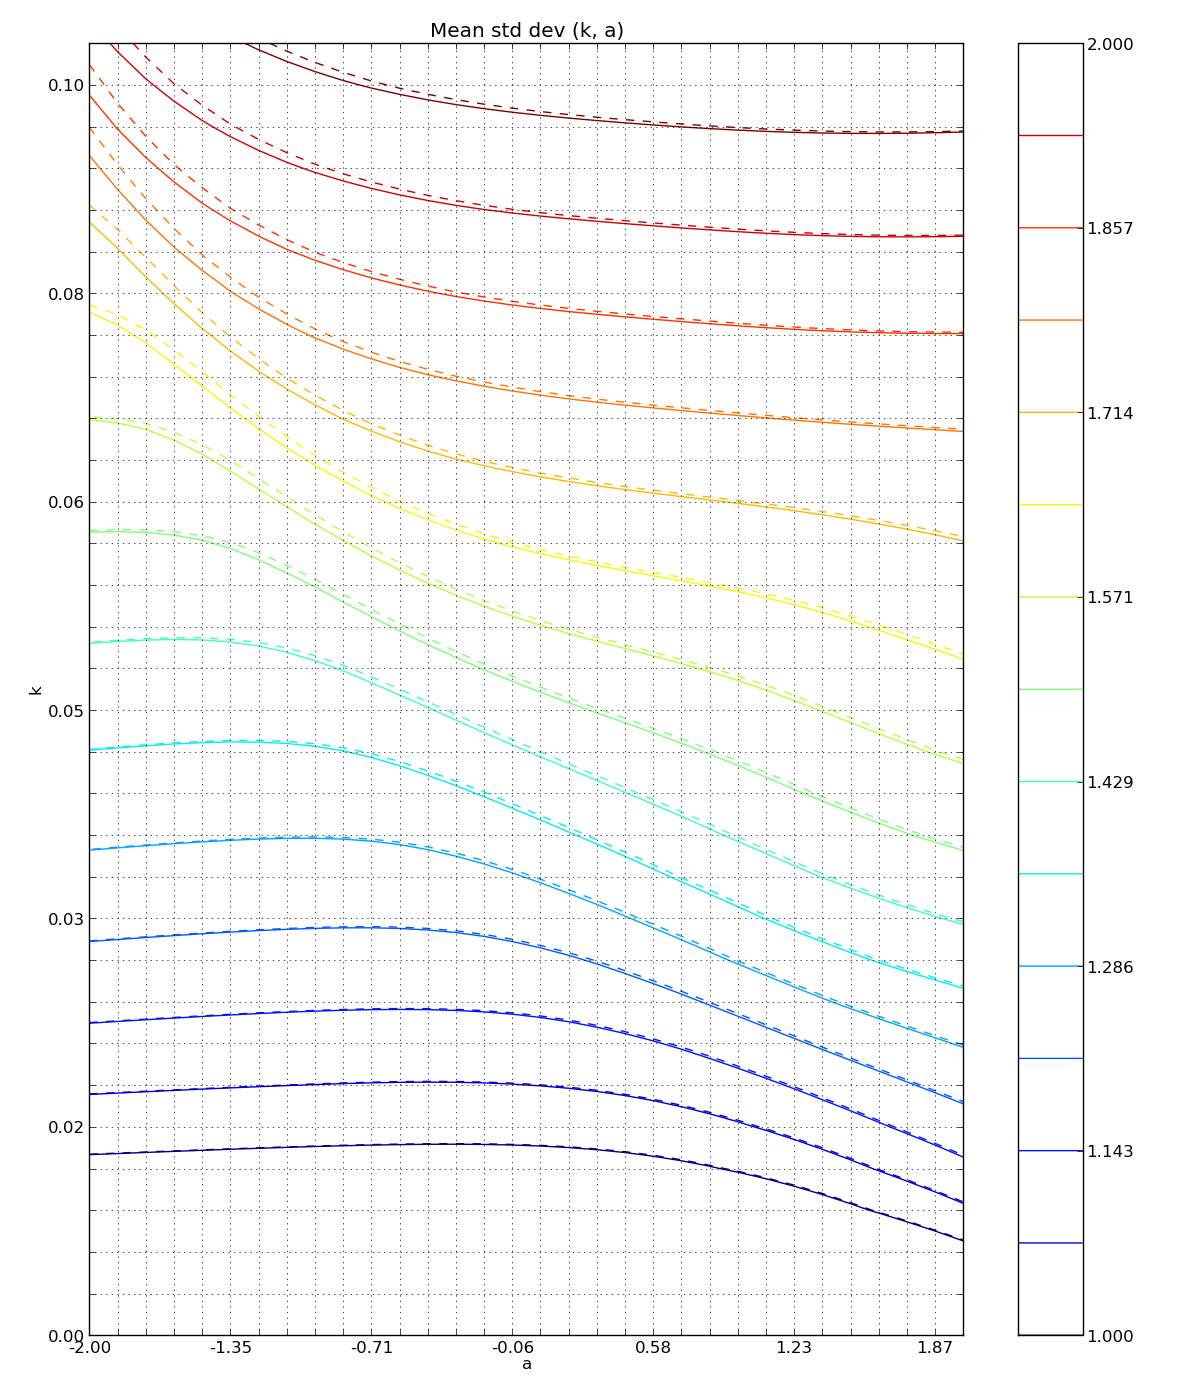
\includegraphics[width=0.48\textwidth]{images/gpu_pse.png}}
		\caption{}
		\label{fig:gpu_pse}
	\end{figure}

	As can be seen in the listing, the calculations
	in native code are performed with 32-bit floating point numbers, and it
	is reasonable to ask if this is numerically accurate. In Fig 
	\ref{fig:gpu_pse}, we present a parameter space exploration performed with
	both the pure Python NumPy simulator and the GPU simulator, showing the 
	isocontours of average standard deviation in the parameter space. Some
	deviation can be identified visually in parts of the parameter space, and
	in in Fig \ref{fig:gpu_dxdt}, we show in more detail time series of 
	the Python and GPU solutions.

	 \begin{figure}
		{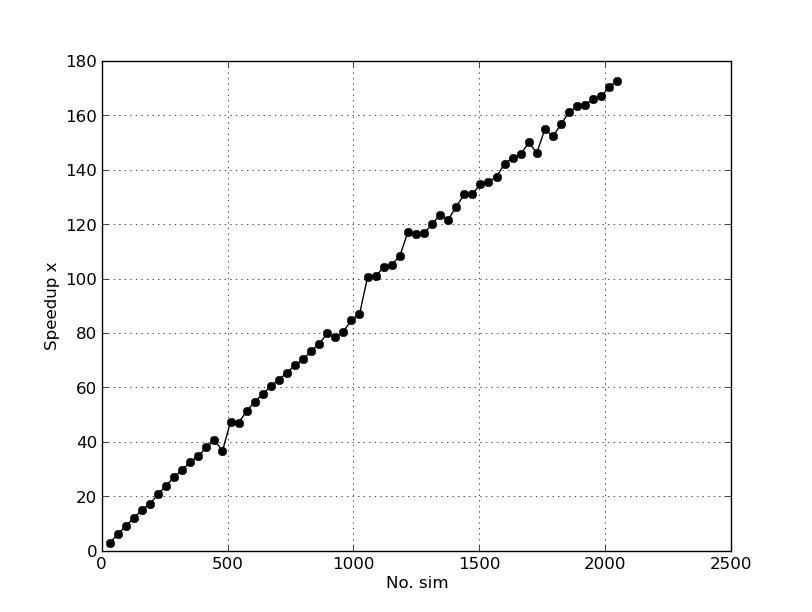
\includegraphics[width=0.48\textwidth]{images/gpu_acceleration.png}}
		\caption{}
		\label{fig:gpu_pse}
	\end{figure}

	This approach allows significant acceleration of parameter sweeps in the
	case of the GPU by taking
	advantage of the fact that in many cases, only numerical values vary
	between different threads and not memory access patterns. Where one of the
	dimensions of a parameter sweep implies changing memory access patterns, 
	for example conduction velocity, it is advantageous to reorder the parameters,
	so that such memory varying parameters only change between grids of GPU
	threads and not within.

	In Fig \ref{fig:gpu_acceleration}, we plot the speedup brought by the GPU
	over the Python NumPy simulator as a function of the number of simulations 
	performed simulataneously on the GPU.



\subsection{Other simulators compared to \TVB}

	Brian should be a particular focus in this section, as it may
	be one of the closest. 

	- several spiking models in the literature use the notain of a reset
		condition and potential, for which Brian provides explicit
		functionality. TVB does not because typically the deterministic
		dynamics of neural mass models are continuous.
